\section{Results}\label{sec:results}

\subsection{Sigma Hyperparameter Selection}\label{subsec:sigmaHyperparameterSelectionResults}
Recall that $\sigma_1, \sigma_2, \ldots \sigma_n$ are hyperparameters that must be defined prior to executing the
algorithm.
The grid search exhausts every permutation $P_n^{\sigma_n}$, where:
\begin{equation}
    \label{eq:gridSearchQuerySigma}
    \sigma_n \ \in \ \{10^{-16}, 10^{-15}, \ldots 10^{1}\}
\end{equation}
% 2.22 * 10^-16 is the machine epsilon for double

\begin{figure*}
    \centering{
    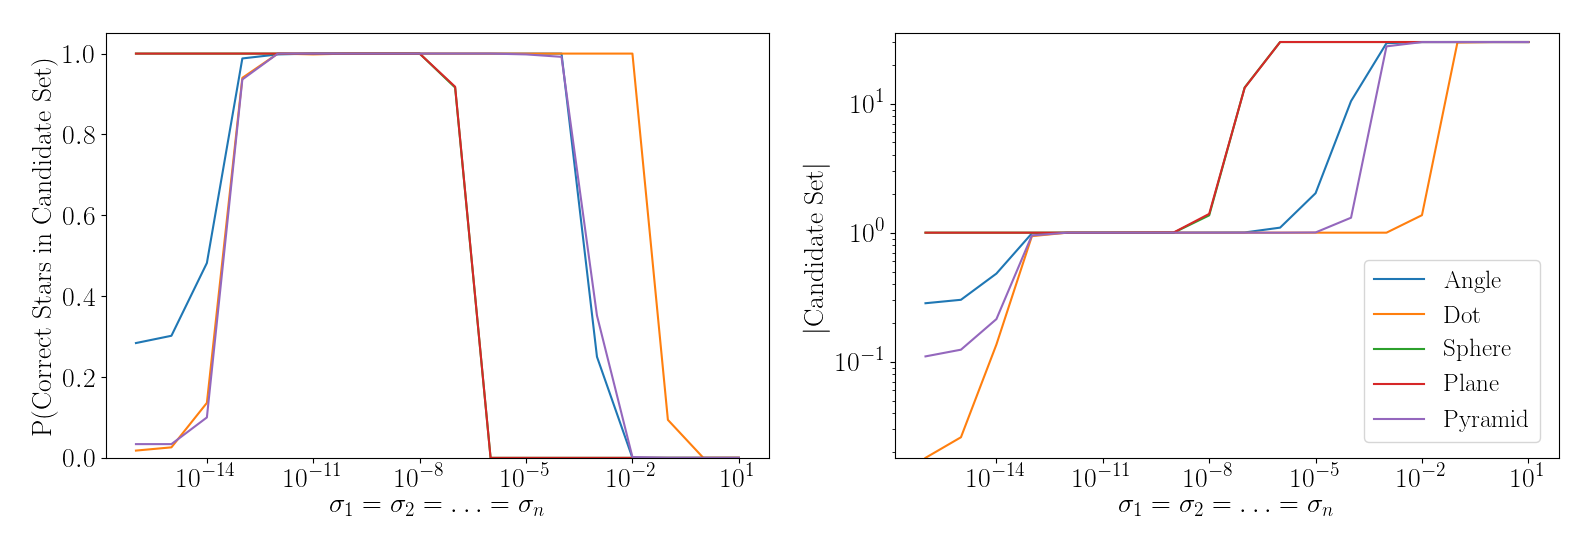
\includegraphics[scale=0.45]{images/sigma1-pcss-css.png}
    \caption{
    The left plot depicts the effect of varying $\sigma$ on the probability that the correct star set exists in the
    resulting candidates after the query.
    The right plot depicts the effect of varying $\sigma$ on the average size of the candidate set after the query, bounded
    by 30 candidates at maximum.
    The field-of-view is bounded by $f = 20^\circ$ and the apparent magnitude is bounded by $m = 6.0$.
    Each point represents the average of 1000 query steps without noise introduced.
    For brevity, all deviations associated with methods of more than one feature term (i.e.\ Dot Angle, Spherical
    Triangle, \ldots) had all corresponding $\sigma$ terms set equal to each other.
    } \label{figure:sigmaHyperparameterPlots}
    }
\end{figure*}

The set of plots in~\autoref{figure:sigmaHyperparameterPlots} depict the effect on different $\sigma$ terms against the
average size of the candidate set $S$ (on the left) and the probability that the correct stars exist in this candidate
set $Q$ (on the right).
If the deviation is too small, then the selectivity of each query becomes too restrictive and no results are returned.
On the other hand when the selectivity is too high, the candidate set size upper bound of 30 candidates is
hit and the chance that the correct candidate exists in the query declines.

The ideal period for all methods identifying images restricted by $f < 20 \land m < 6.0$ occurs when:
\begin{equation}
    \label{eq:idealRegionAcrossFeatures}
    \sigma_n \ \in (10^{-12}, 10^{-8})
\end{equation}
Regardless of the feature, a deviation choice between these bounds should be acceptable for distinguishing stars.

% Not including this, don't feel it is relevant to ideal analysis.
%It is important to note that each feature exists in different bounds.
%The values below represent the observed bounds of each feature:
%\begin{alignat*}{2}
%    \label{eq:observedFeatureSpace}
%    % Non-inclusive bounds given below.
%    \theta^{ij} &\in (2.6 \times 10^{-3} &&, 2.0 \times 10^1) \\
%    \theta^{ij} &\in  (2.6 \times 10^{-3} &&, 2.0 \times 10^1) \\
%    \theta^{ic}, \theta^{jc} &\in (2.6 \times 10^{-3} &&, 2.0 \times 10^1) \\
%    \phi &\in (1.3 \times 10^{-3} &&, 1.8 \times 10^2) \\
%    a^{ijk} &\in (3.1 \times 10^{-9} &&, 5.4 \times 10^{-2}) \\
%    \imath^{ijk} &\in (4.8 \times 10^{-16} &&, 5.3 \times 10^{-4}) \\
%    a^{ijk} &\in (3.7 \times 10^{-9} &&, 5.3 \times 10^{-2}) \\
%    \imath^{ijk} &\in (4.9 \times 10^{-16} &&, 5.3 \times 10^{-4})
%\end{alignat*}

% TODO: Replace these values with the ones using the most recent dataset.
\begin{table}
    \centering {
    \caption{
    Ideal query hyperparameter determination and sensitivity results of each method.
    The ideal region length $\ell$ represents the number of deviations where~\autoref{eq:idealQuery} is held.
    Each method's critical points $\sigma_{c1}$ and $\sigma_{c2}$ a is the upper bound on the $Q$ and $S$
    ideal region.
    } \label{tab:sensitivityIdealResults}
    \begin{tabular}{m{0.27\columnwidth}|m{0.13\columnwidth}|m{0.2\columnwidth}|m{0.2\columnwidth}}
        \textbf{Method} & $\ell$ & $\frac{\partial Q}{\partial\sigma} \text{ at } \sigma_{c1}$ &
        $\frac{\partial S}{\partial \sigma} \text{ at } \sigma_{c2}$ \\
        \hline \hline
        \textbf{Angle} & 3 & -0.375 & 0.001 \\ \hline
        \textbf{Dot Angle} & 9 & -0.453 & 0.183 \\ \hline
        \textbf{Spherical \newline Triangle} & 8 & -0.042 & 0.181\\ \hline
        \textbf{Planar \newline Triangle} & 6 & -0.041 & 0.001 \\ \hline
        \textbf{Pyramid} & 7 & -0.001 & 0.002
    \end{tabular}
    }
\end{table}

Referencing~\autoref{tab:sensitivityIdealResults}, there appears to some correlation between the number of
\textit{distinct} features and length of the stability region here.
The Dot Angle method uses three total features, two of which are distinct from each other ($\theta$ vs. $\phi$) for
it's query.
The Pyramid method uses three similar features, which has the same stable region length as the triangle methods
using two distinct features.
The Angle method uses only one feature for its query, and suffers in stable region length.

The candidate set size responses are most likely a result of the size of possible candidates that belong to each
method's respective feature (i.e.\ the number of rows of the table used in query).
The Angle method has the least number of possible candidates given the $f < 20 \land m < 6.0$ constraint, at 353700
possible catalog sets.
The triangle methods have roughly 35 times as many possible catalog sets as the Angle method.
The Dot Angle method has 3 times as many possible catalog sets as the triangle methods, and roughly 105 times as many
possible catalog sets as the Angle method.
Given a larger pool of results to choose from, it follows that the number of false positive increases as well.

The largest $Q$ response belongs to the Dot Angle method, while the smallest response belongs to the Pyramid method.
Unlike the candidate set size response, there appears to be no obvious correlation between the response of correct
star set existence and the number of features used.
If noise is not known, the most forgiving feature set in terms of both responses is the Pyramid method.

The $\sigma$ parameters for the following experiments were chosen using the results of the grid search, and selecting
the largest $\sigma_1, \sigma_2, \sigma_3$ (ordered as such) that maintained all the
conditions in~\autoref{eq:idealQuery}.
\begin{alignat*}{2}
    \text{Angle}&: \sigma_\theta &&= 1.0 \times 10^{-4}\\
    \text{Pyramid}&: \sigma_\theta &&= 1.0 \times 10^{-4}\\
    \text{Dot Angle}&: \sigma_{\theta_{ic}} &&= 1.0 \times 10^{-1}\\
    \text{Dot Angle}&: \sigma_{\theta_{jc}} &&= 1.0 \times 10^{-1}\\
    \text{Dot Angle}&: \sigma_\phi &&= 1.0 \times 10^{-3} \\
    \text{Spherical Triangle}&: \sigma_a &&= 1.0 \times 10^{-1}\\
    \text{Spherical Triangle}&: \sigma_\imath &&= 1.0 \times 10^{-11}\\
    \text{Planar Triangle / Composite}&: \sigma_a &&= 1.0 \times 10^{-1} \\
    \text{Planar Triangle / Composite}&: \sigma_\imath &&= 1.0 \times 10^{-11}\\
\end{alignat*}

In addition to the $\sigma_n$ parameters used in the previous experiments, a parameter $\sigma_o$ must be defined
prior to executing the \Call{DMT}{} method.
The linear search exhausts every overlay deviation selection:
\begin{equation}
    \label{eq:linearSearchSigmaOverlay}
    \sigma_n \ \in (10^{-16}, 10^{2})
\end{equation}

\begin{figure*}
    \centering{
    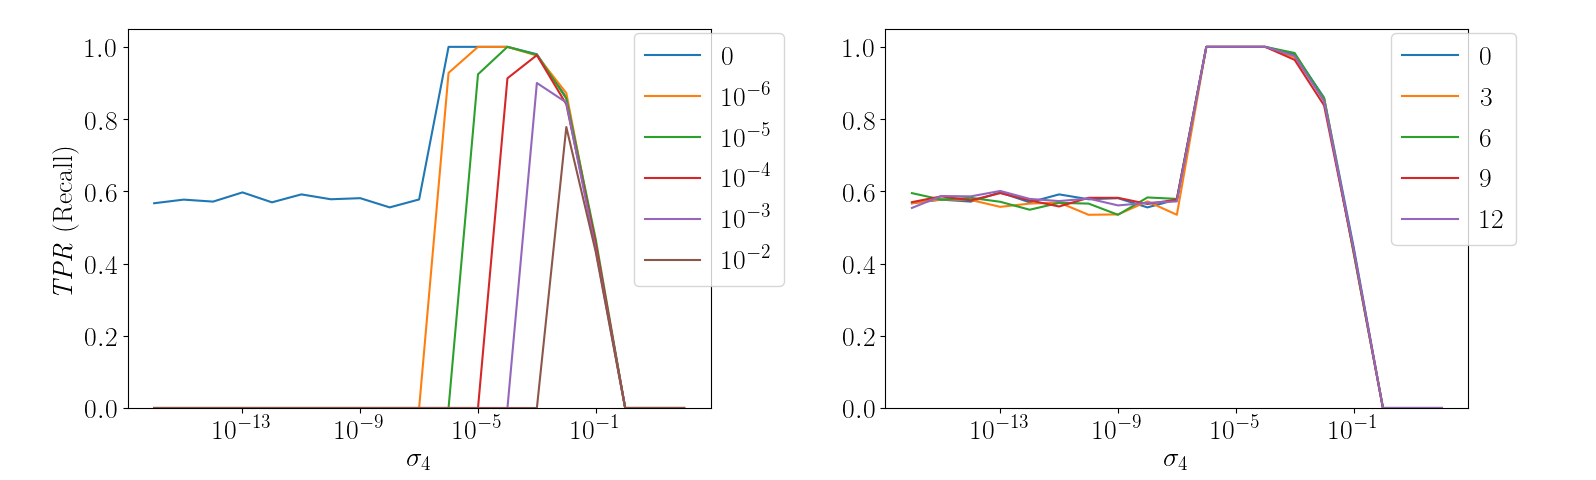
\includegraphics[scale=0.45]{images/sigma4-recall.png}
    \caption{
    Both plots depict the effect of varying $\sigma$ on the recall.
    The left plot depicts this relationship for different variations in noise, while the right plot depicts the same
    relationship for different numbers of false stars.
    The field-of-view is bounded by $f = 20^\circ$ and the apparent magnitude is bounded by $m = 6.0$.
    Each point represents the average of 200 query steps.
    } \label{figure:sigmaOverlayHyperparameterPlots}
    }
\end{figure*}

The set of plots in~\autoref{figure:sigmaOverlayHyperparameterPlots} depict the effect on different $\sigma$ terms
against the recall.
The period of accurate stability for Gaussian noise under $\sigma = 10^{-5}$ and for all false star introductions occurs
when:
\begin{equation}
    \label{eq:sigmaOverlayStableRegion}
    \sigma_4 \ \in (10^{-6}, 10^{-3})
\end{equation}

% TODO: Fix this here.
Looking at the both plots it is interesting to note that under no noise (Gaussian or false stars), a $\sigma_4 \ \in
(10^{-17}, 10^{-6})$ gives a recall of $~0.57 \pm 1.8 \times 10^{-2}$.
In this region, it appears that the \ldots
On the other end of the stability period for $\sigma_4 > 10^0$, accuracy drops straight to 0 regardless of the noise
presented.
At this period, stars are labeled with more weight to the order of the stars in the image rather than actually falling
within the specified deviation.

Focusing on the left plot of varying Gaussian noise, the accuracy dips to zero once the deviation of Gaussian noise
exceeds the selected deviation.
Past the $10^{-4}$ mark, the largest accuracy a deviation choice can achieve is no longer equal to one.
If noise is known, then the appropriate deviation for the \Call{DMT}{} method can be selected.
The right plot shows that the accuracy is not affected under different amounts of false stars.
Given varying amounts of false stars, virtually none of these stars were identified as an actual star.
The \Call{DMT}{} method is seen as highly specific, yielding no false positives.

The value of $\sigma_4 = 10^{-4}$ was selected for use in the \Call{DMT}{} method.
This is the largest deviation that lies in the accurate stable region.

\subsection{Query Selectivity}\label{subsec:querySelectivityResults}
Using the optimal hyperparameters described in the previous section, each query step was analyzed in terms of its
$Q$ and $S$ response to an introduction of Gaussian noise.

%\begin{figure*}
%    \centering{
%    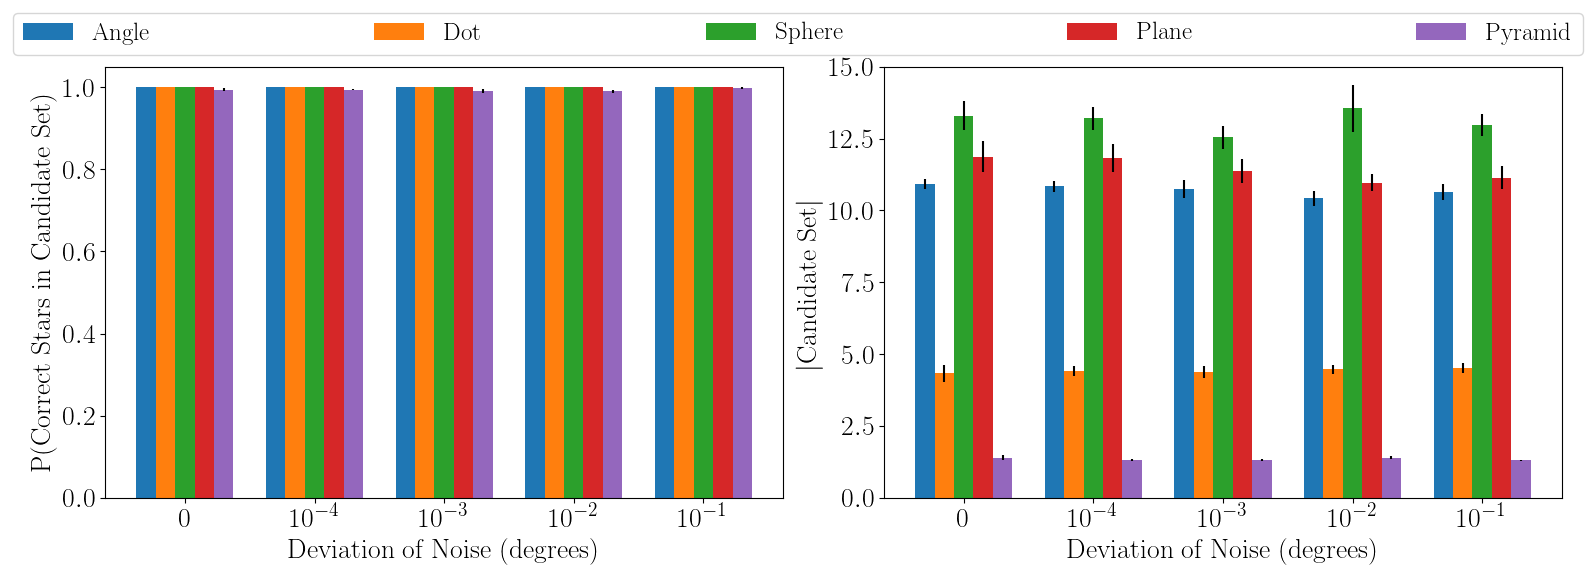
\includegraphics[scale=0.45]{images/query-exp.png}
%    \caption{
%    The left plot depicts the effect of varying the deviation of Gaussian noise on the probability that the correct
%    star set exists in the resulting candidates after the query.
%    The right plot depicts the effect of varying this same noise on the size of the candidate set after the query,
%    bounded by 5000 candidates at maximum.
%    Field of view limit is $f = 20^\circ$.
%    Each point represents the average of 5000 query steps.
%    For the probability measure these 5000 steps were split into 1000 averages, and the mean of these averages are
%    presented above.
%    } \label{figure:queryPlots}
%    }
%\end{figure*}

\begin{table}
    \centering {
    \caption{
    Each method's probability that the correct star set exists after querying ($Q$) and average candidate set size ($S$)
    under the presence of Gaussian noise.
    Every star in the image presented to each identification method's querying process was shifted toward some
    random direction, whose magnitude was normally distributed by $\sigma=0.1^\circ, \mu = 0^\circ$.
    Each point represents the average of 5000 query steps.
    } \label{tab:queryExperimentResults}
    \begin{tabular}{m{0.18\columnwidth}|m{0.34\columnwidth}|m{0.34\columnwidth}}
        \textbf{Method} & $Q$ & $S$ \\
        \hline \hlinescore
        \textbf{Angle} & $1.000 \pm 0.00 $ & $10.90 \pm 1.96 \times 10^{-1}$ \\ \hline
        \textbf{Dot Angle} & $1.000 \pm 0.00 $ & $04.52 \pm 1.08 \times 10^{-1}$ \\ \hline
        \textbf{Spherical \newline Triangle} & $1.000 \pm 0.00 $ & $12.84 \pm 6.61 \times 10^{-1}$ \\ \hline
        \textbf{Planar \newline Triangle} & $1.000 \pm 0.00 $ & $11.43 \pm 2.46 \times 10^{-1}$ \\ \hline
        \textbf{Pyramid} & $0.994 \pm 6.63 \times 10^{-3}$ & $01.31 \pm 2.20 \times 10^{-2}$
    \end{tabular}
    }
\end{table}

In~\autoref{tab:queryExperimentResults}, each method's $Q$ and $S$ is displayed under the presence of noise.
It is important to note that the data for the same experiment without the introduction of noise is very similar to that
with noise, suggesting that Gaussian noise does not affect the outcome of the query step.
Any inaccuracies with the overall identification process are most likely a result of future steps.

All methods are able to produce no false negatives after the query step except for the Pyramid method, whose accuracy
dips very slightly.
On the other hand, the Pyramid method consistently produces the smallest average candidate set size.
By sacrificing $Q$, the Pyramid method ensures a smaller average candidate set size.
This tradeoff can only be made when there exists other stars to choose from, as star trackers with a small number of
stars to choose from will be left without other combinations to identify stars from.

The next smallest average candidate set size can be seen with the Dot Angle method (5 candidates), followed by the
Angle method (11 candidates), and the triangle methods (13 for Spherical, 12 for Planar) last.
Feature sets involving angular separation are more selective than those using triangular features.

The most selective feature set that does not sacrifice accuracy is the Dot Angle.

\subsection{Candidate Reduction}\label{subsec:candidateReductionResults}
Using the same optimal hyperparameters described in~\autoref{subsec:sigmaHyperparameterSelectionResults}, each query +
reduction step was analyzed in terms of the average accuracy and efficiency response to Gaussian noise and false stars.

\begin{figure*}
    \centering{
    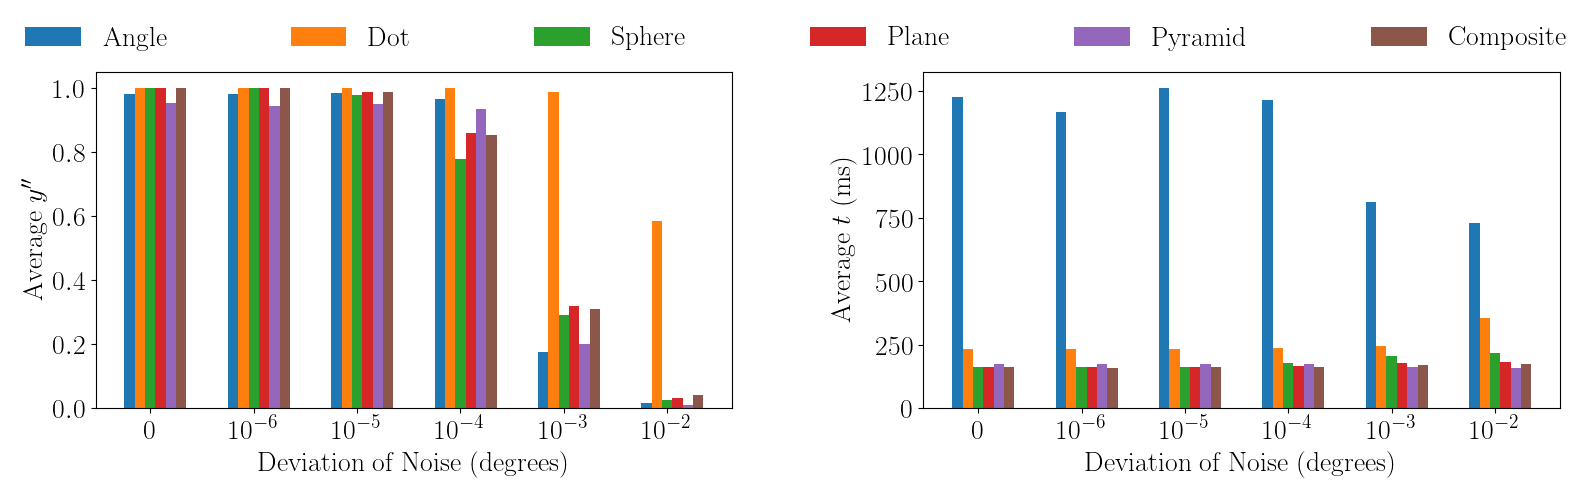
\includegraphics[scale=0.45]{images/reduction-shift-exp.png}
    \caption{
    Both plots depict the effect of varying the deviation of Gaussian noise on the average accuracy (left) and
    average number of query steps to get an answer (right) for different identification methods.
    The field-of-view is bounded by $f = 20^\circ$ and the apparent magnitude is bounded by $m = 6.0$.
    Each point represents the average of 100 reduction steps.
    } \label{figure:reductionShift}
    }
\end{figure*}

Without noise in both~\autoref{figure:reductionShift} and~\autoref{figure:reductionFalse}, only the triangle methods
had XXX\% accuracy in reduction.
The process of pivoting is also fairly inexpensive without noise, using no more than XXX steps on average
(or, XXX pivot step) to obtain a reduction set.
On the other end the Composite Pyramid is the least accurate and least efficient on average, using XXX steps to
obtain an accuracy of XXX\%.
Both of these methods use the triangular features, but the triangular pivoting process is vital in using catalog
candidate sets with both true and false positives catalog sets.
The Composite Pyramid method instead restricts it's catalog candidate sets to the set $\{R \mid 1 = |R| \}$, which
wastes query steps to find a unique result.

The second worst, which barely beats the Composite Pyramid in both accuracy (XXX\%) and efficiency (XXX query steps) is
the Angle method.
3rd in accuracy (XXX\%), but 4th in efficiency (XXX query steps) is the Dot Angle method.
The trade-off in catalog candidate size for accuracy from the Pyramid method's query step can be seen in effect here as
the method ranks 1st in efficiency (1 query step), but 4th in accuracy (XXX\%).

In~\autoref{figure:reductionShift}, the deviation of Gaussian noise against the average accuracy and efficiency is
displayed for different identification methods.
As soon as Gaussian noise of $10^{-6}$ degrees is introduced, all methods using triangular features drop to an average
accuracy of XXX\%.
The rest of the methods experience the biggest drop in accuracy for a Gaussian noise of $10^{-3}$ degrees.
The two main reasons for this later noise response are most likely the hyperparameters chosen, and the triangular
features themselves not being distinctive enough.

The hyperparameters for all methods were chosen without any noise introduced.
The upper bound of the ideal region for the angular separation feature was around $\sigma = 10^{-4}$.
It follows that any noise greater than this should lead to a decline in accuracy (average of XXX\% decrease), which
is seen in both the Pyramid and Angle methods.
The Dot Angle method shows an earlier and smaller response (XXX\%) given Gaussian noise of $10^{-4}$ degrees.
These methods have identical reduction steps, suggesting that this is a result of the Dot Angle's $\phi$ feature.

The Spherical / Planar Triangle methods have different reduction steps and features than the previous three methods,
and the response to noise is more severe (average of XXX\% decline).
Part of this may be due to the pivoting process, but seeing a similar decline in the Composite Pyramid method
(average of XXX\% decline) argues that this may be a result of the triangular features themselves.
Increasing the accuracy here is possible by increasing $\sigma$, although~\autoref{tab:queryExperimentResults} shows
that triangular features already yield the highest number of candidates.
Increasing the deviation here would produce even more results, leading to a less efficient reduction process.
What can be said here, is that the triangular features are highly sensitive to Gaussian error at the reduction step.

Looking at the query step count plot on the right, only the Dot Angle method shows no response to noise
(average of XXX query steps).
An introduction of $10^{-6}$ degree noise to the Planar and Spherical Triangle methods leads to an average increase of
XXX query steps.
Seeing as the accuracy drops here for the two methods, it follows that the methods should iterate until all
query sets are exhausted.

The Pyramid method has a very small response to query step count (XXX steps) as accuracy drops around noise of
$10^{-3}$ degrees, and continues to gradually grow for $10^{-2}$ degrees.
As seen in~\autoref{tab:queryExperimentResults} there are less catalog candidates, so the time to catalog candidate
exhaustion is quicker.
The Composite Pyramid method has an interesting decline in the number of query steps, with an average of XXX query
steps at $10^{-6}$ degree noise.
The time to catalog candidate exhaustion is smaller, but accuracy is still at XXX\%.

\begin{figure*}
    \centering{
    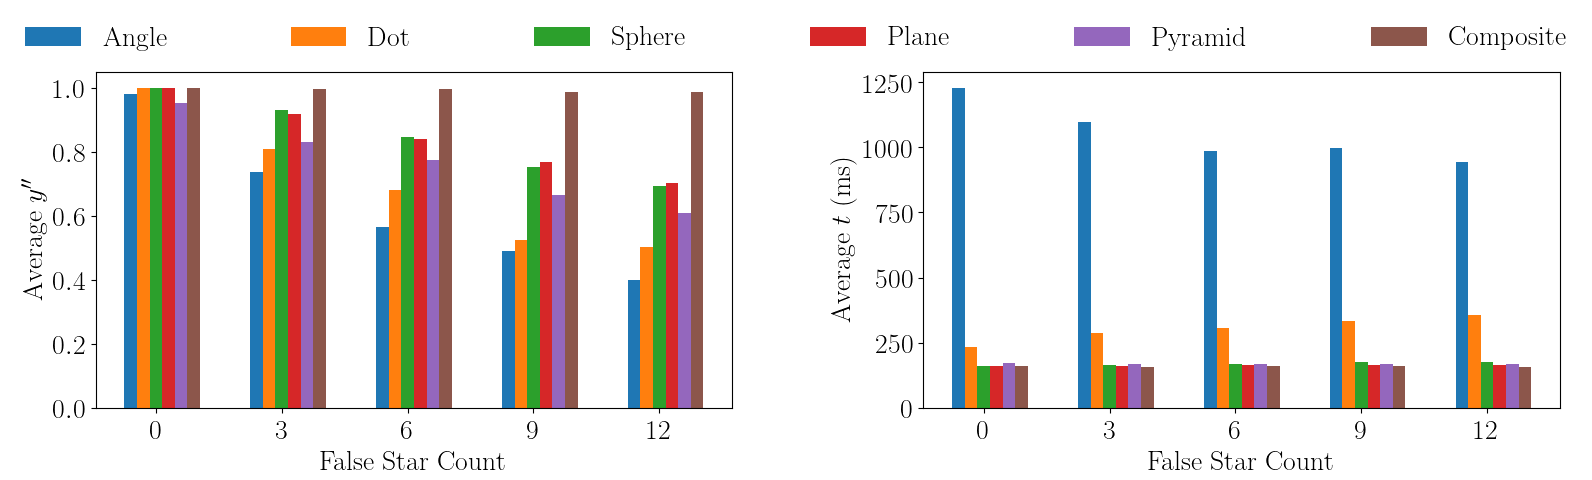
\includegraphics[scale=0.45]{images/reduction-false-exp.png}
    \caption{
    Both plots depict the effect of varying the number of false stars on the average accuracy (left) and
    average number of query steps to get an answer (right) for different identification methods.
    The field-of-view is bounded by $f = 20^\circ$ and the apparent magnitude is bounded by $m = 6.0$.
    Each point represents the average of 100 reduction steps.
    } \label{figure:reductionFalse}
    }
\end{figure*}

In~\autoref{figure:reductionFalse}, the number of false stars against the average accuracy and efficiency is displayed
for different identification methods.
It is easier to observe a trend in the noise here.
The number of false stars is generally proportional to the number of query steps, and inversely proportional
to the accuracy.
On the left graph, the Pyramid method has the best accuracy (XXX\%) under the most noise.
The Pyramid method specifies a false star persistence avoidance method for choosing query star sets from the image, and
the effectiveness of this can be seen.
The Composite Pyramid uses the same false star persistence avoidance method, but the difference in features render this
technique less effective than all other identification methods.
While completely accurate under no noise, the Spherical and Planar Triangle methods drop to XXX\% accuracy given
12 false stars.

On the right graph, the Pyramid method uses the least number of query steps to get a catalog set (XXX steps at most).
This again, is most likely a result of the false star persistence avoidance method and the low number of candidates
found at query time.
The Dot Angle method ranks 2nd in average efficiency here (XXX query steps at most), followed by the triangle methods
(mean of XXX query steps at most).
The Angle and Composite Pyramid rank last in efficiency.

As a whole the triangular reduction process works best for images with little to no noise, and the candidate set size
restriction reduction works better otherwise.
The pivot process itself may work better with other features, but anything beyond this is speculation.

Under both types of noise, the best average accuracy to efficiency ratio belongs to the Pyramid method.

\subsection{Identification Determination}\label{subsec:identificationDeterminationResults}
Using all optimal hyperparameters described in~\autoref{subsec:sigmaHyperparameterSelectionResults}, each identification
was ran end-to-end and analyzed in terms of its response to an introduction of Gaussian noise and false stars.

\begin{figure*}
    \centering{
    % TODO: Replace this with the identification image.
    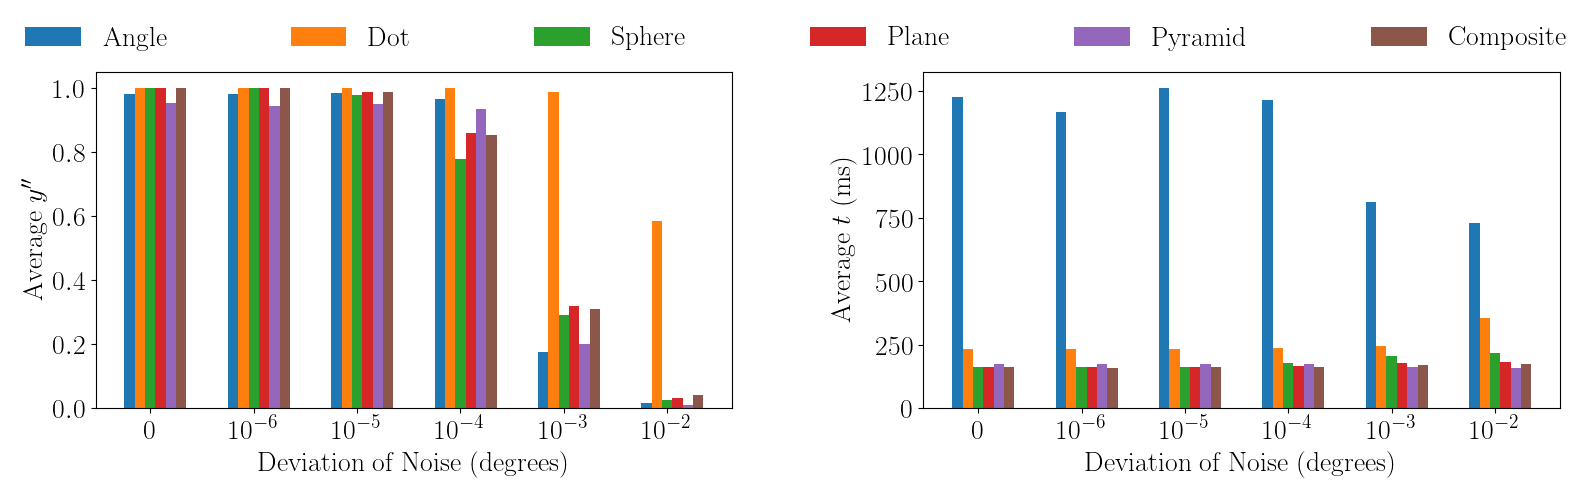
\includegraphics[scale=0.45]{images/reduction-shift-exp.png}
    \caption{
    Both plots depict the effect of varying the deviation of noise on the average accuracy (left) and average number
    of reduction steps to get an answer (right) for different identification methods.
    The field-of-view is bounded by $f = 20^\circ$ and the apparent magnitude is bounded by $m = 6.0$.
    Each point represents the average of 100 identification steps.
    } \label{figure:identificationShift}
    }
\end{figure*}

Without noise in both~\autoref{figure:identificationShift} and~\autoref{figure:identificationFalse}, all methods except
for the Angle and Composite Pyramid yield 100\% accuracy.
The Pyramid method was the most efficient here, with an average of 1 reduction step to obtain an answer.
The Spherical and Planar Triangle methods are 2nd and 3rd in efficiency, consuming an average of 3 reduction steps.
The Dot Angle requires an average of 7 reduction steps, followed by the Angle method at 50 reduction steps and the
Composite Pyramid method at 80 reduction steps.

Remember that all methods except the Dot Angle and Pyramid method rely on the \Call{DMT}{} function to determine how
the catalog set maps to the image set.
Seeing as how the Spherical and Planar Triangle methods larger differ in both measures, it is safe to say that this
function performs as well as the identification process in the Pyramid and Dot Angle method.

In~\autoref{figure:identificationShift}, the deviation of Gaussian noise is displayed against the average accuracy and
efficiency.
When noise of $10^{-6}$ degrees is introduced, all methods decline XXX\% on average in accuracy.
Previously in the reduction experiment, accuracy declined near to zero for the Spherical and Planar Triangle methods.
Low accuracy there, but accuracy on-par here shows a strong $r$ confidence decision step for these methods.
On the other end, the Composite Pyramid always iterates to the $\tau = 100$ limit beyond this, showing that the
candidate reduction step for this method is not able to produce a confident result in a reasonable amount of time.

When noise of $10^{-5}$ degrees is introduced, all methods decline further to an average of XXX\% accuracy.
This contrasts the Dot Angle, Angle, and Pyramid accuracy non-response to Gaussian noise in the reduction experiment.
These methods have the correct catalog set, but are mismapping this to the image set.
% TODO: Finish this shiet here

\begin{figure*}
    \centering{
    % TODO: Replace this with the identification image.
    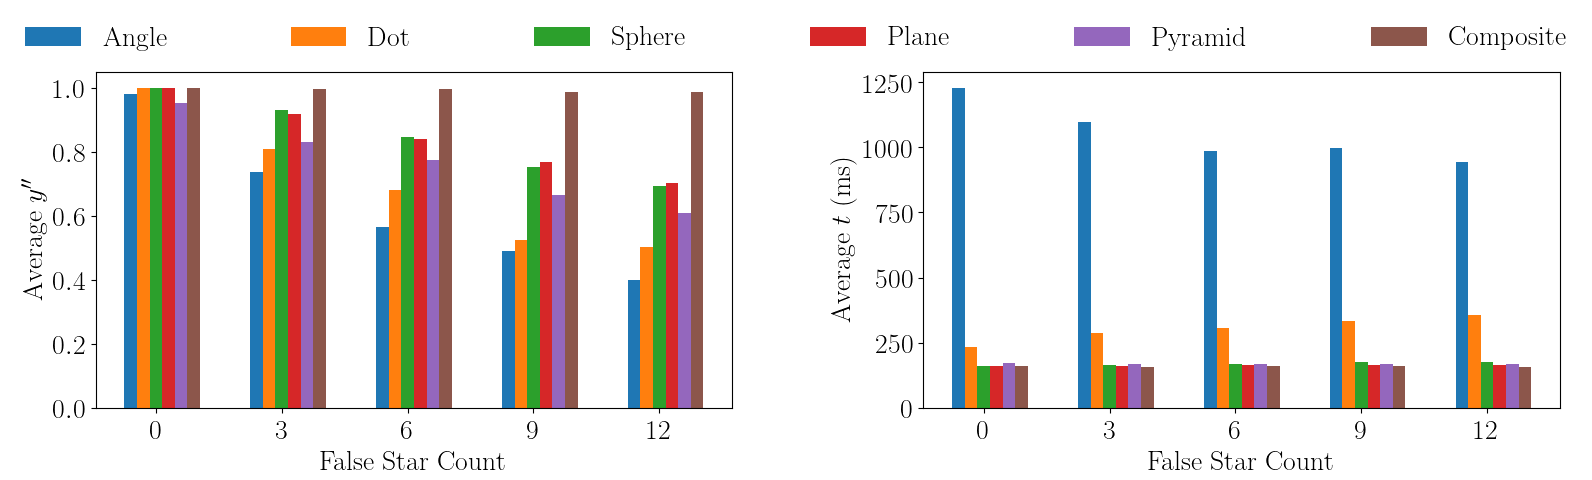
\includegraphics[scale=0.45]{images/reduction-false-exp.png}
    \caption{
    Both plots depict the effect of varying the number of false stars on the average accuracy (left) and average number
    of reduction steps to get an answer (right) for different identification methods.
    The field-of-view is bounded by $f = 20^\circ$ and the apparent magnitude is bounded by $m = 6.0$.
    Each point represents the average of 100 identification steps.
    } \label{figure:identificationFalse}
    }
\end{figure*}

